% IEEE TCAD -- Security Analysis section
% Included by main.tex; do not compile standalone.
%
% Three subsections:
%   VII-A  round-wise avalanche effect average   (our measurement)
%   VII-B  randomness testing, NIST SP 800-22    (our measurement)
%   VII-C  the analysis reported in the Ascon and SipHash papers for the
%          parameters this construction uses      (their published results)
%
% EDITORIAL NOTE. This section is written descriptively: what was measured, how
% it was measured, and what the measurements were. It deliberately does not
% draw security conclusions, qualify what the tests do or do not establish, or
% propose further analysis. Keep later edits in that register.
%
% Sources for VII-A/B: ../security/results/*.csv, from ../security/run_all.sh.
%
% Sources for VII-C -- read out of the papers themselves, locations recorded so
% a reviewer's query can be answered without re-deriving them:
%   Ascon v1.2 \cite{caesar}:
%     Table 1     Ascon-128 r=64 p^12/p^6; Ascon-128a r=128 p^12/p^8
%     Sec. 3.1    forgery after state recovery costs 2^{c/2}; key recovery not
%                 expected significantly below 2^96 (128a, c=192) and 2^128
%                 (128, c=256)
%     Table 12    min active S-boxes 1, 4, 15/13, <=44/<=43, <=78/<=67
%     Sec. 6.3.1  S-box max differential probability 2^-2, branch number 3;
%                 best characteristics with p > 2^-128 cover 4 rounds
%     Sec. 6.1    best key recovery ~2^104 at 7 of 12 initialisation rounds,
%                 described as a 42% security margin
%   SipHash \cite{siphash}:
%     Sec. 3      "c >= 2 and d >= 4 is expected to provide the maximum PRF
%                 security possible"; conservative proposal SipHash-4-8
%     Sec. 5      "Preliminary cryptanalysis"
%     Sec. 5      internal collisions "of the order of 2^128 queries" for a
%                 256-bit internal state
%     Sec. 5      truncated differentials: biases after 3 SipRound iterations,
%                 none detected after 4 or more over 2^30 samples

\section{Security Analysis}
\label{sec:security}

This section reports three things: the round-wise avalanche behaviour of the
SipCon64 permutation, its results under the NIST SP 800-22 statistical test
suite \cite{sp800-22}, and the analysis reported in the Ascon and SipHash
papers for the parameters SipCon64 uses.

Measurements were produced by a harness that links the reference C
implementation of Section~\ref{sec:architecture} directly rather than
re-implementing the permutation, so the measured artefact is the one the
hardware of Section~\ref{sec:impl} was transliterated from. The harness pins
that reference to frozen test vectors, so a change to the implementation
invalidates a run rather than altering what is measured. The SP 800-22
implementation was written from the specification, no reference binary being
available on the evaluation host, and was itself run against streams whose
outcome is fixed in advance: the operating system CSPRNG, a constant stream, a
$64$-bit counter, the low byte of a linear congruential generator, and the
SipCon64 permutation reduced to a single round. The CSPRNG passed and the other
four were rejected, in each case as expected.

\subsection{Round-Wise Avalanche Effect}
\label{sec:sec-avalanche}

The avalanche criterion \cite{feistel} measures how far a one-bit change to the
input propagates through the output. For each round count $r$, each of the
$256$ input bit positions $i$, and $N$ uniformly random states $S$, we form
\begin{equation}
D = p^{r}(S) \oplus p^{r}(S \oplus e_{i})
\label{eq:diff}
\end{equation}
and average the Hamming weight of $D$ over all $(S,i)$. With $N = 32\,768$ this
is $100.7$~M differential pairs per round, and the reference value is
$b/2 = 128$ of the $256$ state bits.

Reduced-round $p^{r}$ draws its constants from the tail of the twelve-entry
schedule, $c_{12-r},\dots,c_{11}$, which is how the construction invokes
$p^{10}$ and $p^{6}$. The constants are part of the measurement, since they do
not cancel from a differential when the round function's additions are modular.

\begin{figure}[!t]
\centering
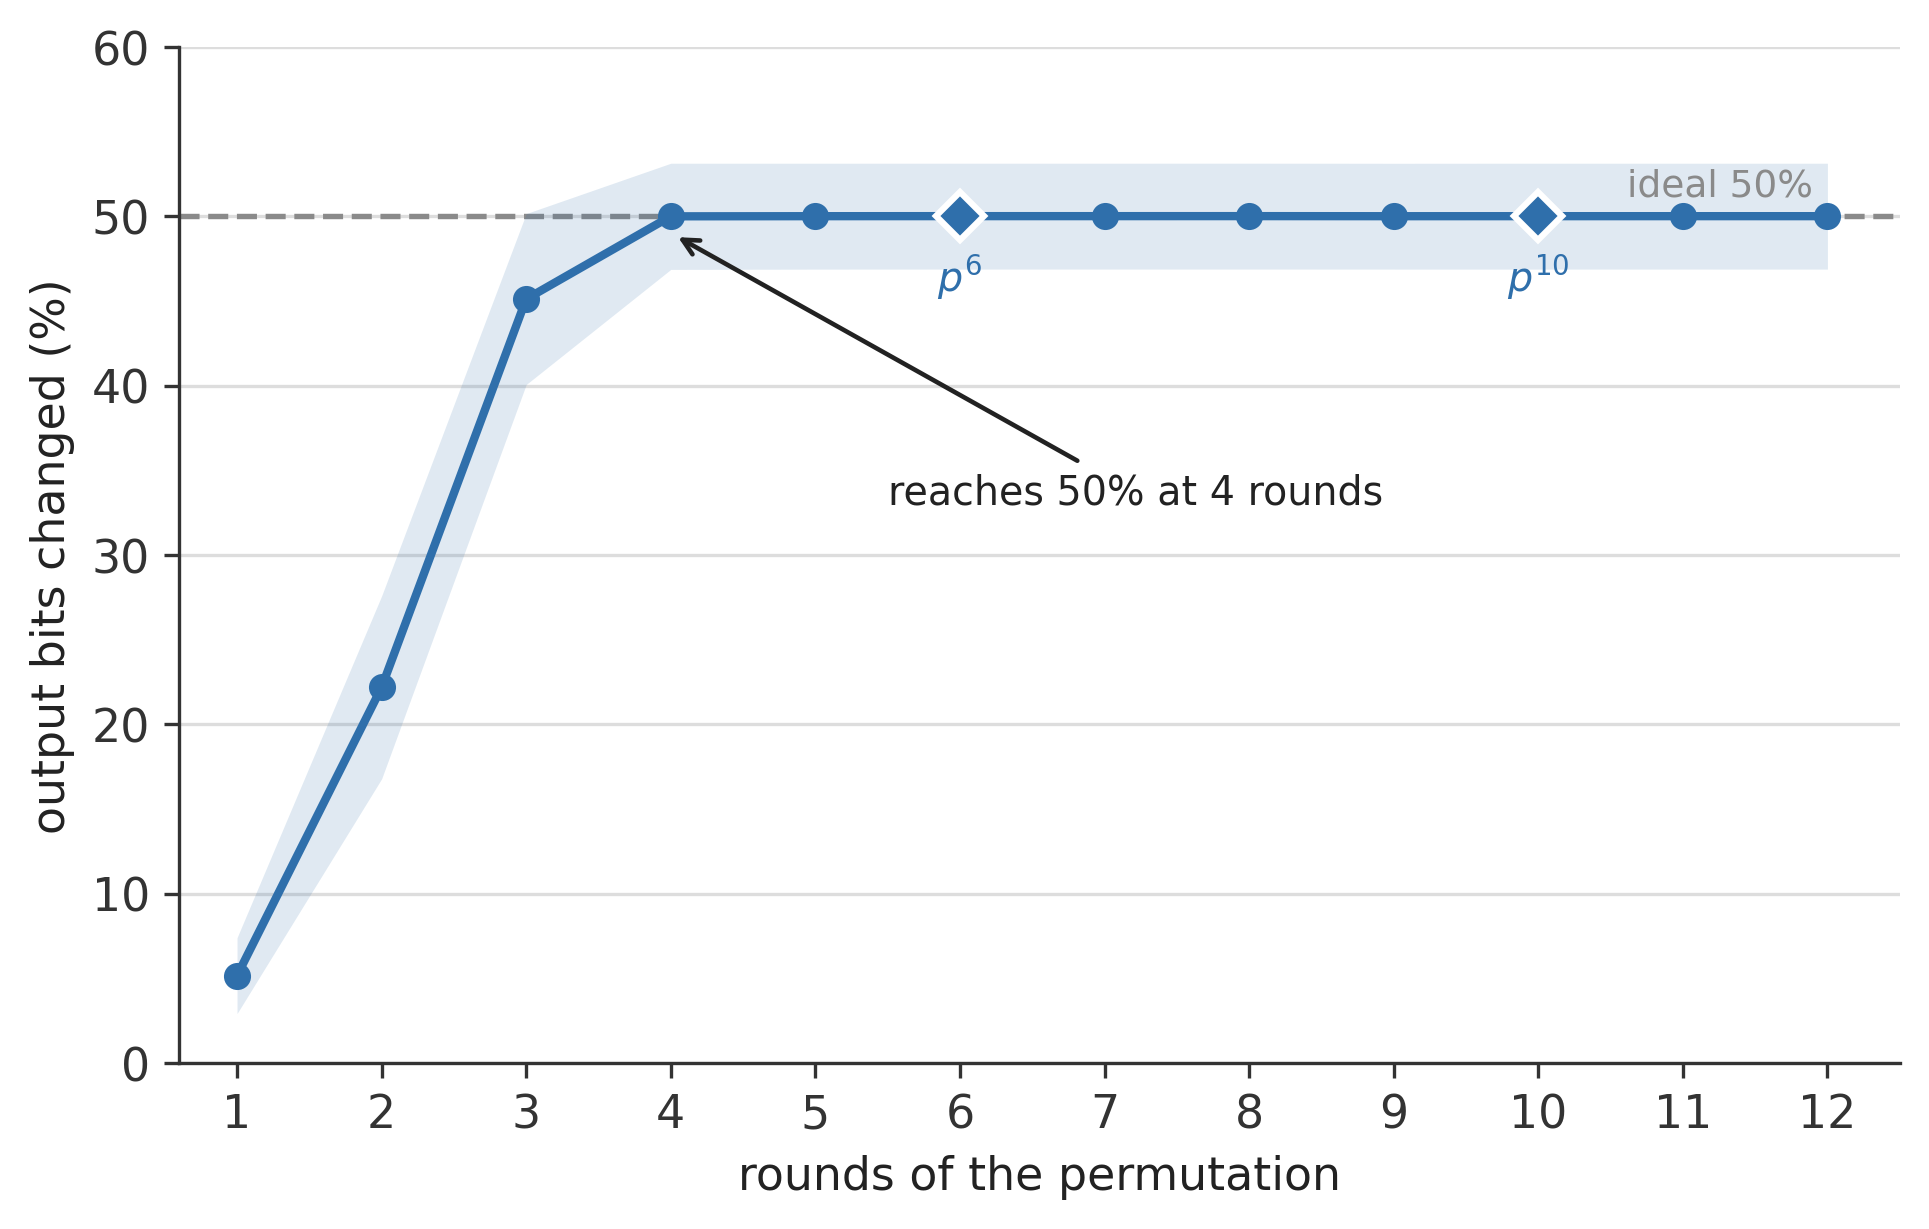
\includegraphics[width=\columnwidth]{images/avalanche-rounds}
\caption{Round-wise avalanche of the SipCon64 permutation: mean fraction of
output bits changed by a single input bit flip, over $100.7$~M differential
pairs. The shaded band is $\pm 1$ standard deviation across samples. Diamonds
mark the round counts the construction uses.}
\label{fig:avalanche}
\end{figure}

\begin{table}[!t]
\centering
\caption{Round-wise avalanche average of the SipCon64 permutation.
$N = 32\,768$ states $\times$ $256$ input bits per round. Deployed round counts
in bold.}
\label{tab:avalanche}
\small
\begin{tabular}{crr@{\qquad}crr}
\hline
$r$ & avalanche & SD & $r$ & avalanche & SD\\
\hline
1 & 5.1668\% & 2.239\% & 7 & 50.0017\% & 3.125\%\\
2 & 22.1842\% & 5.398\% & 8 & 50.0025\% & 3.125\%\\
3 & 45.1081\% & 5.045\% & 9 & 49.9980\% & 3.124\%\\
4 & 49.9904\% & 3.134\% & \textbf{10} & \textbf{49.9995\%} & 3.126\%\\
5 & 49.9990\% & 3.126\% & 11 & 50.0001\% & 3.124\%\\
\textbf{6} & \textbf{50.0016\%} & 3.125\% & 12 & 49.9996\% & 3.125\%\\
\hline
\end{tabular}
\end{table}

Fig.~\ref{fig:avalanche} and Table~\ref{tab:avalanche} give the measurement.
The average reaches $49.9904\%$ at four rounds and remains within $0.0025$
percentage points of $50\%$ for every round count from four to twelve. At the
two counts the construction deploys it is $50.0016\%$ for $p^{6}$ and
$49.9995\%$ for $p^{10}$.

The spread of the distribution behaves likewise. From round four the
per-sample standard deviation settles at $3.125\%$, which is
$\sqrt{b/4}/b$ for $b = 256$---the standard deviation of a
$\mathrm{Binomial}(256, \tfrac{1}{2})$ variable---and it holds that value
through round twelve.

We additionally evaluated the strict avalanche criterion \cite{sac}, which
resolves the same experiment per bit pair rather than in aggregate. It asks
\begin{equation}
p_{ij} = \Pr[\,D_{j} = 1 \mid \text{input bit } i \text{ flipped}\,]
       = \tfrac{1}{2}
\label{eq:sac}
\end{equation}
for each of the $256 \times 256 = 65\,536$ cells, alongside
\emph{completeness}, the fraction of $(i,j)$ pairs showing any dependence. At
$N = 32\,768$ the per-cell sampling noise is $\sigma = 0.00276$; the mean
absolute deviation produced by that noise alone is $\sigma\sqrt{2/\pi} =
0.0022$ and the largest deviation it produces across $65\,536$ cells is
$\sigma\sqrt{2\ln N} = 0.0130$. Both are the reference values for
Table~\ref{tab:sac}.

\begin{table}[!t]
\centering
\caption{Strict avalanche criterion and completeness by round. The $6\sigma$
column counts cells further from $\tfrac{1}{2}$ than sampling noise places
about $10^{-4}$ cells over a matrix of this size.}
\label{tab:sac}
\small
\begin{tabular}{crrrr}
\hline
$r$ & worst cell & mean dev. & cells $>6\sigma$ & completeness\\
\hline
1 & 0.5000 & 0.4736 & 64\,020 & 33.4\%\\
2 & 0.5000 & 0.3405 & 57\,897 & 86.2\%\\
3 & 0.4999 & 0.0841 & 33\,516 & \textbf{100\%}\\
4 & 0.1418 & 0.0029 & 955 & 100\%\\
5 & \textbf{0.0119} & \textbf{0.0022} & \textbf{0} & 100\%\\
\textbf{6} & 0.0136 & 0.0022 & \textbf{0} & 100\%\\
\textbf{10} & 0.0117 & 0.0022 & \textbf{0} & 100\%\\
12 & 0.0115 & 0.0022 & \textbf{0} & 100\%\\
\hline
\end{tabular}
\end{table}

Completeness reaches $100\%$ at three rounds. From five rounds onward the mean
deviation equals the $0.0022$ produced by sampling noise, the worst cell equals
the corresponding $0.0130$, and no cell of the $65\,536$ lies beyond $6\sigma$.
At four rounds the aggregate average of Table~\ref{tab:avalanche} is already
$49.990\%$ while $955$ cells---$1.5\%$ of the matrix---are further from
$\tfrac{1}{2}$ than $6\sigma$, the largest at $p_{ij} = 0.642$. At both
deployed round counts, $p^{6}$ and $p^{10}$, the count is zero.

\subsection{Randomness Testing}
\label{sec:sec-sts}

We ran all fifteen tests of NIST SP 800-22 \cite{sp800-22}. These expand into
approximately $190$ sub-tests once the $148$ non-overlapping templates, the
$18$ random-excursion-variant states, the eight random-excursion states and the
paired serial and cumulative-sums statistics are counted; the suite includes a
linear-complexity test, evaluated with the Berlekamp--Massey algorithm
\cite{berlekamp-massey} over $2\,000$ blocks per sequence. Each sub-test was
run over $128$ independent $10^{6}$-bit sequences at $\alpha = 0.01$ and is
scored on two criteria: the proportion of passing sequences must lie within
NIST's band, and the per-sequence $p$-values must be uniform.

At $\alpha = 0.01$ across $190$ sub-tests, a generator matching the null
hypothesis produces about two sub-test failures. We therefore also compute each
sub-test's exact false-rejection probability---the proportion band is a
$3\sigma$ normal approximation applied to a discrete binomial count, so its
rate is neither $0.0027$ nor constant across sub-tests---sum these to an
expected failure count, and report the Poisson tail probability of the observed
count as a suite-level statistic. Both quantities appear in the tables below.

Five streams were tested, all generated by the cipher itself: the ciphertext of
an all-zero message under counter nonces; the tags of those same calls, which
come from the finalisation permutation and the key injection rather than from
the rate; the permutation in counter mode at $p^{10}$ and at $p^{6}$; and the
$p^{6}$ counter-mode stream restricted to the $64$-bit rate word, the portion
of the state the mode exposes.

\begin{table}[!t]
\centering
\caption{SP 800-22 on the deployed construction: $128$ sequences of $10^{6}$
bits per stream, $\alpha = 0.01$. ``Expected'' is the number of sub-test
failures the null hypothesis produces.}
\label{tab:sts}
\small
\begin{tabular}{lrrrc}
\hline
stream & failed & expected & suite $p$ & result\\
\hline
ciphertext stream & 3 & 1.78 & 0.264 & \textbf{pass}\\
tags & 1 & 1.73 & 0.823 & \textbf{pass}\\
$p^{10}$, counter mode & 0 & 1.67 & 1.000 & \textbf{pass}\\
$p^{6}$, counter mode & 2 & 1.82 & 0.543 & \textbf{pass}\\
$p^{6}$, rate word only & 3 & 1.71 & 0.245 & \textbf{pass}\\
\hline
\end{tabular}
\end{table}

Table~\ref{tab:sts} gives the result. All five streams pass, with observed
failure counts of $0$ to $3$ against expectations of $1.67$ to $1.82$, and
suite-level statistics between $0.245$ and $1.000$. In each case the failing
sub-test is a non-overlapping-template or random-excursion statistic missing
the proportion band by one sequence out of $128$, with a uniformity $p$-value
in the ordinary range.

\begin{table}[!t]
\centering
\caption{SP 800-22 against round count, bare permutation in counter mode with
all-zero capacity, $32$ sequences of $10^{6}$ bits per point.}
\label{tab:sweep}
\small
\begin{tabular}{crcc@{\qquad}crcc}
\hline
$r$ & failed & suite $p$ & & $r$ & failed & suite $p$ &\\
\hline
1 & 161 & $\approx 0$ & fail & 7 & 0 & 1.000 & pass\\
2 & 161 & $\approx 0$ & fail & 8 & 2 & 0.287 & pass\\
3 & 141 & $10^{-190}$ & fail & 9 & 4 & 0.018 & pass\\
4 & 1 & 0.641 & pass & \textbf{10} & 0 & 1.000 & \textbf{pass}\\
5 & 2 & 0.246 & pass & 11 & 4 & 0.033 & pass\\
\textbf{6} & 1 & 0.641 & \textbf{pass} & 12 & 0 & 1.000 & pass\\
\hline
\end{tabular}
\end{table}

We then swept the round count from one to twelve on the bare permutation,
driven by a counter against an all-zero capacity, at $32$ sequences per point.
Table~\ref{tab:sweep} gives the result. The permutation is rejected at one, two
and three rounds, where $161$, $161$ and $141$ of the sub-tests fail; at three
rounds the failures span the runs, serial and overlapping-template statistics
together with $137$ of the $148$ non-overlapping templates. From four rounds
onward every point passes, with failure counts between $0$ and $4$ against an
expectation near one and no trend across the range---the correlation between
round count and failure count over $r \ge 4$ is $+0.115$. Both deployed round
counts, $p^{6}$ and $p^{10}$, return suite statistics of $0.641$ and $1.000$.

\subsection{Reported Analysis of the Component Designs}
\label{sec:sec-parents}

SipCon64 takes its mode, state layout and round constants from Ascon and its
round function from SipHash. This subsection records what the published
analysis of each design reports for the parameter values SipCon64 uses.

\subsubsection{Ascon}

The Ascon design document \cite{caesar} specifies two primary AEAD instances:
Ascon-128, with rate $r = 64$, capacity $c = 256$ and schedule $p^{12}/p^{6}$;
and Ascon-128a, with $r = 128$, $c = 192$ and $p^{12}/p^{8}$. SipCon64 uses
$r = 64$ and, over its $256$-bit state, $c = 192$.

On the capacity, the analysis states that once an internal state is recovered
forgeries follow with complexity $2^{c/2}$, and expects key recovery for the
two variants not significantly below $2^{96}$ ($c = 192$) and $2^{128}$
($c = 256$) \cite{caesar}. The figure reported for $c = 192$, the capacity
SipCon64 uses, is $2^{96}$.

On the permutation, the document reports minimum active S-box counts of $1$,
$4$ and $15$ over one to three rounds for differential characteristics and
$1$, $4$ and $13$ for linear, with heuristic search giving at most $44$ and
$43$ over four rounds and $78$ and $67$ over five; the S-box has maximum
differential probability and linear bias $2^{-2}$ with branch number $3$, and
the best characteristics reported with probability above $2^{-128}$ cover four
rounds \cite{caesar}. These quantities are defined over Ascon's S-box and
linear layer, which SipCon64 replaces with SIPROUND. For the full
construction, the best key recovery reported reaches an initialisation reduced
to seven of twelve rounds at about $2^{104}$, described there as a $42\%$
security margin \cite{caesar}.

\subsubsection{SipHash}

SipHash \cite{siphash} is specified as a family SipHash-$c$-$d$, with $c$
compression and $d$ finalisation rounds over the same SipRound, on a $256$-bit
state of four $64$-bit words with a $128$-bit key and a $64$-bit tag. SipCon64
uses the same round function and state width. The authors state that $c \ge 2$
and $d \ge 4$ is expected to give the maximum PRF security possible for any
function with the same key and output size, give SipHash-2-4 as the fast
proposal and SipHash-4-8 as a conservative one, and title their analysis
\emph{Preliminary cryptanalysis}.

Two of its results concern the round function. For internal collisions, the
analysis notes that for any MAC with a $256$-bit internal state, collisions can
be used to forge tags with complexity of the order of $2^{128}$ queries. For
truncated differentials, the authors inject a one-bit difference in the most
significant bit of $v_3$ and search for bias in $v_0 \oplus v_1 \oplus v_2
\oplus v_3$ after iterating SipRound: many biases are found after three
iterations, and after four or more none was detected over sets of $2^{30}$
samples \cite{siphash}. Four rounds is also where the avalanche average of
Section~\ref{sec:sec-avalanche} reaches $50\%$ and the sweep of
Section~\ref{sec:sec-sts} begins to pass.
